\documentclass[hyperref,UTF8]{ctexart}    
	\usepackage{amsmath}
	\usepackage{amssymb}	
	\usepackage[a4paper,bindingoffset=0.2in,%
            left=1in,right=1in,top=1in,bottom=1in,%
            footskip=.25in]{geometry}
\usepackage{graphicx}
\usepackage{enumerate}
\usepackage{url}
\usepackage{hyperref}
\usepackage{pbox}
\usepackage{CJKutf8}


\begin{document}
\title{报告}
\author{盛嘉成, 14307130038 \\ 计算机科学与技术学院}
\maketitle
\section{NavieBayes}
\subsection{模型概述}
分类问题即找出使得后验概率$P(y_{i}|x_{1},x{2},...x_{N})$最大的类别$y_{i}$,在本次试验中,观测值为邮件的词频等57个特征值,分类为是否为垃圾邮件的二分类。
\par
根据贝叶斯公式:\[P(y_{i}|x_{1},x{2},...x_{N})\propto P(y_{i})P(x_{1},x{2},...x_{N}|y_{i})\]其中各类别的先验概率比较方便估计,如$P(spam)$为训练集中垃圾邮件个数/训练集总邮件数。而条件概率密度的估计在输入特征的维度较高时就显得比较复杂,此时就需要用到朴素贝叶斯假设,即各维度特征条件独立$P(x_{1},x{2},...x_{N}|y_{i})=P(x_{1}|y_{i})P(x{2}|y_{i})..P(x_{N}|y_{i})$,于是问题转变为求解下式:
\[{\arg\min}_{\i}P(y_{i})\prod_{j=1}^{N}P(x_{j}|y_{i})\]
\par
为了方便计算,同时也考虑到python实现时多个非常小的概率密度相乘会引起的float精度问题,在原式上取对数,变成等价问题:
\[{\arg\min}_{i}(\log P(y_{i})+\sum_{j=1}^{N}\log P(x_{j}|y_{i}))\]
\par 
所以接下问题的核心就是如何更好地估计各个特征分别在好邮件或垃圾邮件条件下的概率,概率分布的模型选择和相应的参数估计方法都将会在具体实现的报告中围绕这一问题展开。
\par 
朴素贝叶斯关于各个输入特征条件独立的假设显然是一个非常强的、一般不成立的假设。离开这个假设,我们就被迫直接估计N维变量的概率分布,这是非常难以计算的,比如我们假设这N维特征的条件概率分布服从n维高斯分布,直接用训练样本对n维高斯函数的2n个参数做相合无偏有效的估计是非常困难的,对于高斯分布这一特例,可以使用协方差矩阵,但整体上离开了朴素贝叶斯的假设,问题的确变得很复杂,好在许多情况下,即使无法精确满足朴素贝叶斯假设,该模型还是有比较好的分类效果。

\subsection{数据预处理}
\par
为了更好的描绘每个独立的特征的条件概率,除了选取合适的概率分布模型,数据的预处理也十分重要,实际上预处理和模型选择两者也是息息相关的,比如二值化和beta-bernoulli。
\par
从实验中我感受到,进行预处理的一个好处在于,通过干预特征值的数值本身的分布,在条件概率估计之前融入了人的常识,比如,当我们对词频这个特征进行二值化,这就意味着我们假设对于区分好邮件或垃圾邮件,某些单词出现与否,比出现频率更值得关心。(在之后的试验中,发现这个假设很可能是成立的)
\par
具体二值化、归一化、取对数各个预处理的差距和可能的选择原因将在高斯朴素贝叶斯模型中具体讨论。
\par 
朴素贝叶斯带来的另一个好处是我们能独立的处理每个特征的概率分布,比如词频和capital-run-length-average等特征的数值分布、对分类的重要性等都有着本质的区别,由此我们可以对不同的特征进行不同处理(时间关系并未在代码中实现)。

\subsection{Beta-Bernoulli分类器}
\par
对二值分布,我们可以使用伯努利模型,容易证明,样本中1出现的频率是参数$\mu = P(x=1)$的相合无偏有效估计,进一步我们为$\mu$引入先验概率分布,为了满足共轭性,我们引入Beta分布,就得到了Beta-Bernoulli模型。相应的参数估计方法如下:
\par
由书上公式(2.17),并且加入$y_{i}$的条件,我们可以得到:
\[P(\mu |m,l,a,b,y_{i})\propto \mu^{m+a-1}(1-\mu)^{l+b-1}\]
\par 其中m和l分别为在属于类$y_{i}$的样本中观测到1和0的数量。
\par
寻找最好的$\mu$,即找最大化上式的$\mu$,为此将上式取对数:
\[ (m+a-1)\log \mu+(l+b-1)\log (1-\mu)\]
\par 求导,令导数等于0:
\[\frac{m+a-1}{\mu}-\frac{l+b-1}{1-\mu}=0\]
\par 得到:
\[\mu=\frac{m+a-1}{m+l+a+b-2}\]
\par 根据实验要求,我们假设a=b,令n=m+l为某一类样本总数,所以我们得到最好的条件概率估计:
\[P(x_{j}=1|y_{i})=\frac{m_{i}+a-1}{n_{i}+2a-2}\]
\[P(x_{j}=0|y_{i})=1-\frac{m_{i}+a-1}{n_{i}+2a-2}\]

\par
确认参数估计后,我们就确认了beta-bernoulli下朴素贝叶斯分类的算法。该算法计算简单,速度比之后的高斯模型快很多,效果明显更好,由此可见我们第二节关于二值化的假设是合理的。
\par
最后,讨论一下超参a的影响:
\par
令a=b,实际上就是意味着我们认为$\mu$的先验的期望是$E(\mu)=\frac{a}{a+b}=0.5$,当a越大,这个先验对$\mu$的整体参数估计影响越大,从实验结果来看,这个先验估计并不理想。
\par
同时我们也观察到分类器在test集上表现反而比train集上表现更好,可能是因为对于train集,用样本中x=1出现的频率估计概率本来就是最好的估计,用beta分布施加影响反而适得其反。
\\
\begin{table}[!htbp]
% \resizebox{1.4\linewidth}{!}
  \centering
  \scalebox{1}{
\begin{tabular}{ l || c | c | c }
  \hline      
  alpha & 1 & 10 & 100   \\ \hline
  Train-Err. \%  & 11.2 & 11.9 &14.0   \\
  Test-Err. \%  & 11.0 & 11.3 &13.2   \\
  \hline  
\end{tabular}
}
\caption{不同$\alpha$下错误率}
\label{tb:lda_knn}
\end{table}

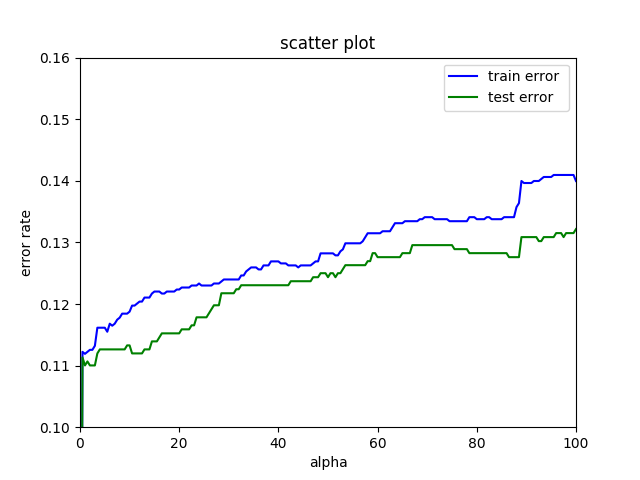
\includegraphics{alphaerror.png}

\par
一个小优化:鉴于$\mu$的计算非常方便更新,在测试时可以不断把测试样例归入训练集,更新参数估计。(经过实验这个优化的实际效果比较有限,对于大部分a,优化后比优化前只多分对了一至两份邮件)


\subsection{高斯分类器}
\par
对于大部分生活中有着复杂因素的连续变量,用高斯分布表达概率密度可以说是不二选择。
\par
高斯分布的参数估计是显然的,用均值估计$\mu$,,用样本标准差估计$\sigma$(为了方便也可以直接用标准差代替),然后我们自然地得到每个特征的条件概率分布,这个过程无需赘述。
\par 
得到每个特征在不同类下的条件概率后,我们同样取对数求和,得到最大化后验概率的估计,这个过程和beta-bernoulli模型比,由于每次要计算高斯函数,使得其效率大大低于后者。
\par
需要注意一个细节,由于某个特征可能是一个类中的所有邮件都具备同样值的(尤其是二值化以后),样本方差可能为0,但是参数$\sigma$不能为0,所以当样本方差为0,我们改用一个极小的值代替,实验中使用了0.001。
\par
主要通过高斯模型来讨论一下预处理的问题,由于高斯函数的值域为实数集,没有预处理的必须性,但是实践证明,预处理对分类效果有良好的提升,除了给定的预处理方法,自己测试了两种二值化方法。
\par 无预处理:效果一般。
\par log: 取对数的意义在于,对于某些特征,其特征值中零散地分布了小部分特别大的值,乃至大大提高了均值和方差,此时的高斯分布就不能很好的估计特征的条件概率,取对数可以使得分布相对集中,一定程度上解决这个问题。
\par z-normalization: 在高斯模型中,这个预处理仅仅相当于把每个特征在每个类下的高斯分布归一化为标准高斯分布,从结果来看意义不明显。
\par 简单二值化:简单的二值化,看上去非常粗糙,而且对于本次实验而言,相当于舍弃了几个最小值为1的特征,但是实验表明,即使这样,二值化使得某些单词是否出现这一特征突显了出来,得到了比较好的结果,再次印证了之前的假设。
\par 通过均值或中位数二值化:直觉上觉得通过均值或者中位数作为阈值二值化相比简单二值化更能因地制宜的考虑样本本身表现的属性,而且不会舍弃任何一个特征。而比较均值和中位数,和取对数的考虑相同,方差过大的数据分布中基于均值的二值化失去了把特征分为强弱两类的效果,实践也表明通过中位数做阈值二值化在本次试验的数据上有着最好的表现。

\begin{table}[!htbp]
% \resizebox{1.4\linewidth}{!}
  \centering
  \scalebox{1}{
\begin{tabular}{ l || c | c | c | c | c | c | c | c | c | c}
  \hline      
  preprocessing & none & log & z-norm & binary & bin-mean & bin-median \\ \hline
  Train-Err. \%  & 17.5 & 16.3 &17.5 &13.8 &17.7 &12.1  \\
  Test-Err.  \% & 18.6 & 18.0 &18.8 &15.7 &18.2 &14.5  \\
  \hline  
\end{tabular}
}
\caption{不同预处理在高斯模型中的错误率}
\label{tb:lda_knn}
\end{table}



\bibliographystyle{plain}
\bibliography{report}


\end{document}